% !TEX root = ../main.tex

\chapter{基于随机博弈模型的分布式动态任务分配框架}
\label{chap:stochastic}

\section{引言}
\label{sg:intro}

第\ref{chap:pg}章和第\ref{chap:hedonic}章是针对静态场景下的任务分配问题,但在解决第\ref{chap:model}章中提出的动态场景下的任务分配问题时,会面临两大问题:一是环境动态变化难以预测,如出现导弹通信网络变化,或目标数量可能出现变化等情况,使得求解模型中的重要变量,如任务效用函数发生变化,原纳什均衡被破坏;二是前两章提出的利用博弈理论提出的决策算法,由仿真结果可知最终收敛结果与收敛速度具有一定的波动性,实际上与算法开始迭代时的初始解有关。

为了解决以上问题,本章利用随机博弈模型建立了分布式动态任务分配框架,并结合前两章的模型与算法,实现动态环境下的任务分配,并通过仿真结果验证了该框架具有较好动态自适应性。

\section{随机博弈模型}
\label{sg:stochastic_game}

随机博弈模型一般是有多个参与者参与的具有状态概率转移的动态博弈过程。下面的定义给出了随机博弈的概念。

\begin{definition}[随机博弈]
	随机博弈可用一组元组表示$\mathcal{G}=<N,\Omega,\{S_i,U_i\}_{i\in N},q>$,其中$N=\{1,2\dots,n\}$表示博弈参与者集合;$\Omega$表示模型所有的可能状态集合;对于每个可能状态$\omega \in \Omega$,都有一个与之相关的阶段博弈$\gamma(\omega)$,该博弈具有策略空间$S^\omega$和效用空间$U^\omega(s)$;$q(\omega^{t+1}|\omega^t,s)$是状态转移概率,表示在$t$时刻模型状态$w^t$下,参与者选择策略$s$后,模型在$t+1$时刻转移到状态$w^{t+1}$的概率。
\end{definition}

随机博弈一般具有多个阶段,在每个博弈阶段,博弈模型会处在一个特定状态中,参与者根据当前状态和预期回报选择自己的最优策略,接着模型会依据状态转移概率转入下一状态,从而开始新一轮博弈。博弈参与者被认为掌握当前状态的信息,且它所能得到的回报仅仅取决于当前状态和它在该状态下采取的策略,而状态转移概率分布完全由当前状态和参与者的决策策略决定。



\section{面向动态任务分配问题的随机博弈框架设计}
\label{sg:framework}

将随机博弈模型应用于导弹任务分配问题,实际上是将某一时刻的任务分配看作是整个模型的状态之一,参与分配的导弹(智能体)即为博弈的参与者,在每个时刻做出的决策即为选择目标。在选择目标后,导弹和目标的飞行会使得环境发生改变,因此下一时刻的任务分配问题便会发生改变。具体而言,本章基于随机博弈模型建立的任务分配框架包含以下几个部分:

(1)状态集合,为每个时刻的任务集合$\mathcal{T}(t), \mathcal{T}(t) \subseteq \mathcal{T}$,$t$为当前时刻;

(2)智能体集合$N=\{1,2\dots,i,\dots,n_m\}$,表示博弈的参与者,每个智能体拥有自己的策略集$\mathcal{A}_i(t) = \{a_k\}$,即为智能体的可选任务集合,且智能体效用函数定义为$U_i(a_i,a_{-i})$;

(3)状态转移概率函数$q(w^{t+1}|w^t)$;

(4)全局效用函数$U_g(a)$。

其中(1)、(2)中的任务集合和智能体集合可直接使用前两章中的概念,使用每个时刻参与分配的导弹和目标集合即可。对于(2)中的智能体效用,本章仍使用第\ref{chap:pg}章中的WLU效用和第\ref{chap:hedonic}章中的效用函数。(3)中的状态转移概率函数取决于模型框架的设计,(4)中的全局效用函数仍沿用前几章的定义。结合第\ref{chap:model}章\ref{model:dynamic_model}小节建立的动态环境模型的特点及可能面临的问题,下面将详细针对模型框架进行阐述。


\subsection{时间窗口划分}
\label{game_stage:time_window}

动态模型下每个时刻环境的状态都与前一时刻不同,一方面不可能对每一时刻建立任务分配模型进行求解,另一方面求解任务分配也需要时间。因此本文将攻击过程划分为若干时间窗口$[t,t+w]$,每一时间窗口作为一个博弈阶段,在同一窗口内,假设导弹和目标态势关系变化不大,最优任务分配结果不会发生改变,因此可以在一个时间窗口内建立起任务分配模型并求解。

时间窗口长度$w$的选取是一个需要权衡的问题。一方面,由于在一个窗口期内,认为态势变化不大,因此如果时间窗口过长,导弹和目标的位置已发生较大变化,态势变化不大的前提假设不再成立,且一些突发事件可能会被忽略而不能及时响应;另一方面,如果时间窗口过短,一方面可能任务分配结果可能还未解出,另一方面鉴于导弹的运动特性,如果频繁重分配可能导致弹道过于弯曲而造成能量浪费。本文后续将通过仿真实验确定时间窗口长度$w$的最优值。

\subsection{博弈子模型建立}
\label{game_stage:submodel}

根据前一小节论述,在划分出一段时间窗口后,需要在每个时间窗口期内建立一个博弈子模型以求解任务分配问题,并且此时可视为静态分配问题求解。因此本小节建立的博弈子模型是基于前两章提出的势博弈分配模型和享乐联盟博弈分配模型。

具体而言,在一个新的博弈阶段开始时,各导弹会根据\ref{model:dynamic_model}小节介绍的模型,统计自己可跟踪的目标以及可通信的导弹,并建立起新的通信网络。根据这些信息,建立势博弈分配模型或享乐联盟博弈分配模型,此时在博弈模型中需要明确各导弹的可选目标集,除了限定为可跟踪到的目标集合$\mathcal{A}^{\text{Detect}}_i$的子集,导弹还需要找出自身可攻击到的目标集合$\mathcal{A}^{\text{Attack}}_i$。结合导弹具有最大过载的特点,本文选择的目标是否可行的判据是:判断导弹攻击该目标所需要的制导过载指令是否会超出导弹的最大过载。设导弹最大过载为$g_{\text{max}}$,导弹在当前状态下攻击该目标预计过载指令为$a_{\text{M}}$,若$a_{\text{M}}>g_{\text{max}}$,则该目标不再是可选目标,所以最终各导弹的可选目标集为$\mathcal{A}_i = \mathcal{A}^{\text{Detect}}_i \cap \mathcal{A}^{\text{Attack}}_i$
。最优分配的求解具体过程与原理前两章已详细阐述,此处不再赘述。

\subsection{博弈阶段切换}
\label{game_stage:stage_transform}

在不同博弈阶段切换的时间点,除了导弹和目标的状态信息、导弹的通信网络发生变化需要更新外,最重要的是任务分配解的传递与切换。根据前面章节的论述和仿真实验可知,在一个博弈阶段内建立的分配模型所得到的最优分配解效果,以及算法收敛速度均与初始解有关。因此在新的博弈阶段子模型建立后,需要决定新的模型下开始算法迭代的初始分配解。如果每次都采用随机生成的解,则每次算法收敛到对应的纳什均衡解会造成时间的浪费,且前文已提到,随机生成的解最终可能得到不同的均衡解,甚至效果较差的均衡解;另一方面,如果一直采用前一阶段的分配解作为新阶段的初始解,则由于原分配解已经是纳什均衡解,且分配模型中的约束条件的存在,可能会限制导弹选择其他目标,使得模型陷入局部最优。

为解决该问题,本文使用的方法是,将前一时刻的分配解与随机生成解以一定概率进行交叉变异,生成新的分配解作为新的博弈阶段的初始解。每个导弹以一定概率$p$选择原分配解$a_k$作为初始解,以$1-p$的概率从$k+1$时刻可选目标集中随机选择一个目标$a_{\text{rand}}^j$作为初始解,则生成$k+1$时刻博弈模型的初始解$a_{k+1}(0)=\{a_{k+1}^1(0),a_{k+1}^2(0),\dots,a_{k+1}^{n_m}(0)\}$

\begin{equation}
\label{sg:eq:crossfactor}
	a_{k+1}^j(0) = I\{e<p\}a_k^j + I\{e \geq p\}a_{\text{rand}}^j,\ e = \mathrm{rand}(0,1).
\end{equation}

此处不需要考虑新解的可行性,因为博弈分配算法会自行消解分配冲突,其中原理前面章节已经论述。

切换过程需要考虑的另一个问题是,在上一个博弈阶段得到的任务分配解,是否接受并传递给下一博弈阶段。由于考虑到频繁切换目标会对导弹带来能量的消耗甚至最终不能成功击中目标,因此本文采用的是带惰性的传递方法,当导弹集群获得$k$时刻的分配结果时,若与当前结果不一致,则会以$q$的概率采用新分配,而以$1-q$的概率拒绝新分配。为了保持分配解的可行性,新分配解的接受或拒绝对所有导弹保持一致,即在同一个连通分支内的所有导弹只要有一枚导弹接受或拒绝新方案,该分支内所有导弹均会作出同样的选择。




\section{事件触发重分配机制}
\label{sg:special_incidence}

虽然在上述随机博弈框架下,假设在一个博弈阶段内态势不会发生重大变化,但实际情况中,发生足以需要重新分配的场景和事件仍是存在的。针对这类突发状况,需要制定一套事件触发机制,明确事件触发信号和触发后重分配方法。

\subsection{通信网络非连通}
\label{special:disconnected_network}

在第\ref{chap:model}章建立的任务分配模型中,导弹存在着通信半径,因此导弹之间建立的通信网络可能存在着非连通的情况。在此情况下,导弹集群往往会形成两个或多个连通分支,无法相互之间共享信息。在此情况下两个不在同一通信分支的导弹可能会生成相互冲突的分配解而无法消除,为了解决这一问题,首先需要引入以下命题。

\begin{proposition}[可消解冲突]
	如果两枚导弹之间不存在通信,则它们在一个博弈阶段内可以消解冲突的条件是
	\begin{equation}
	\label{sg:eq:collision}
		R_{\text{comm}} \geq 2 V_{\text{max}} T_k \Delta t + R_{\text{col}},
	\end{equation}
	其中,$V_{\text{max}}$表示导弹的最大速度,$T_k$表示第$k$个博弈阶段的时间步数,$\Delta t$表示单位时间周期,$R_{\text{col}}$表示导弹碰撞半径。
\end{proposition}

\begin{figure}[!htp]
  \centering
  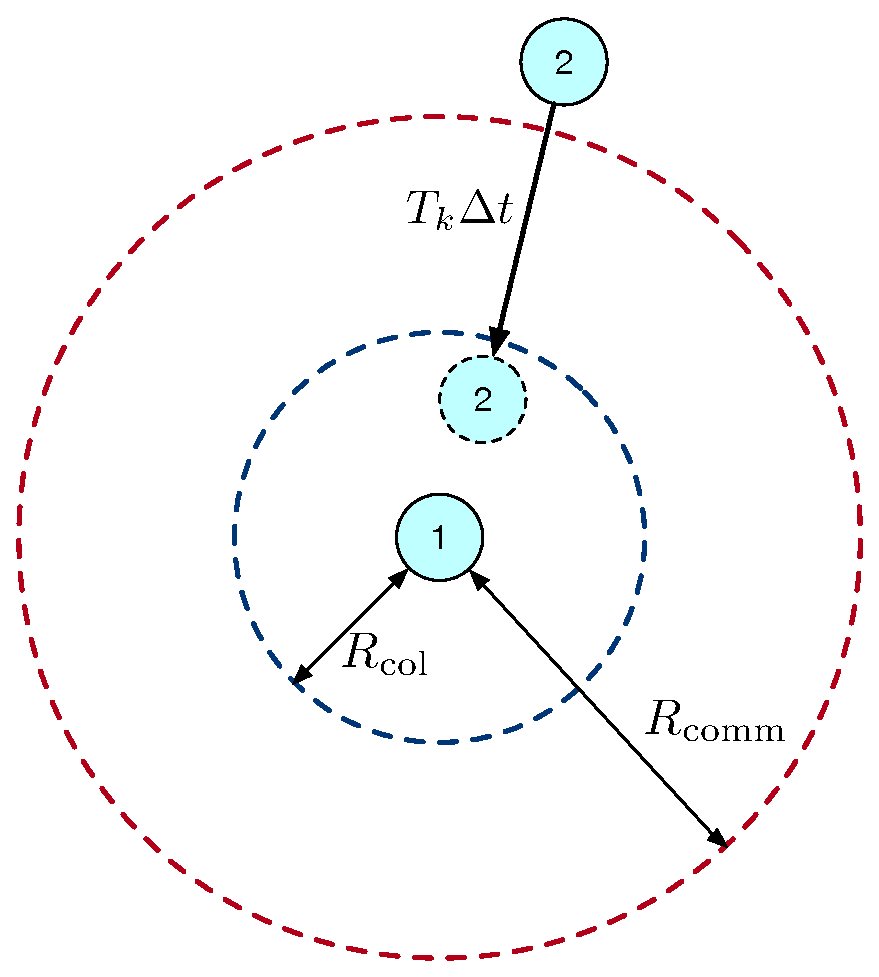
\includegraphics[height=6cm]{stochastic_game/undetectable_collision.eps}
  
  \bicaption[不可规避冲突]
  {不可规避冲突}
  {Illustration of an undetectable collision}
  \label{fig:undetectable_collision}
\end{figure}

在一个时间窗口的博弈阶段内,导弹不会改变分配目标,因此如果出现两个没有建立通信的导弹选择了同一目标产生冲突,则会由于制导律的作用相互靠近,若在时间窗口期内距离小于碰撞距离,则两枚导弹就会发生碰撞,这一过程如图\ref{fig:undetectable_collision}所示,在第k个博弈阶段刚开始时导弹2仍处于导弹1的通信半径(红色虚线圆)外,但在该阶段时间内,导弹2迅速进入了导弹1的最小碰撞半径范围(蓝色虚线圆),此时两导弹难以避免碰撞。

因此为了避免这种情况,对导弹通信半径施加上述条件,使得在同一窗口期内,导弹在碰撞前能够及时建立起通信关系。而新的通信关系一旦建立,会触发重分配条件,原先的分配解在新模型下不再是可行解,从而冲突会被消解,得到的新分配解会适用于新通信网络。这一过程示意图如图\ref{fig:collision_resolution}所示,导弹1和2(蓝色实线实心圆)同时选择了目标1(红色实心圆),但由于互相处于通信范围外(红色虚线圆),并未建立通信,因此冲突无法消解。但随着对目标的接近,两导弹之间的距离逐渐减小(蓝色实心虚线圆),且达到了建立通信的条件,此时触发重分配条件,立即结束当前博弈阶段,建立新的模型重新分配,因此导弹1会重新选择目标2,冲突由此消解。

\begin{figure}[!htp]
  \centering
  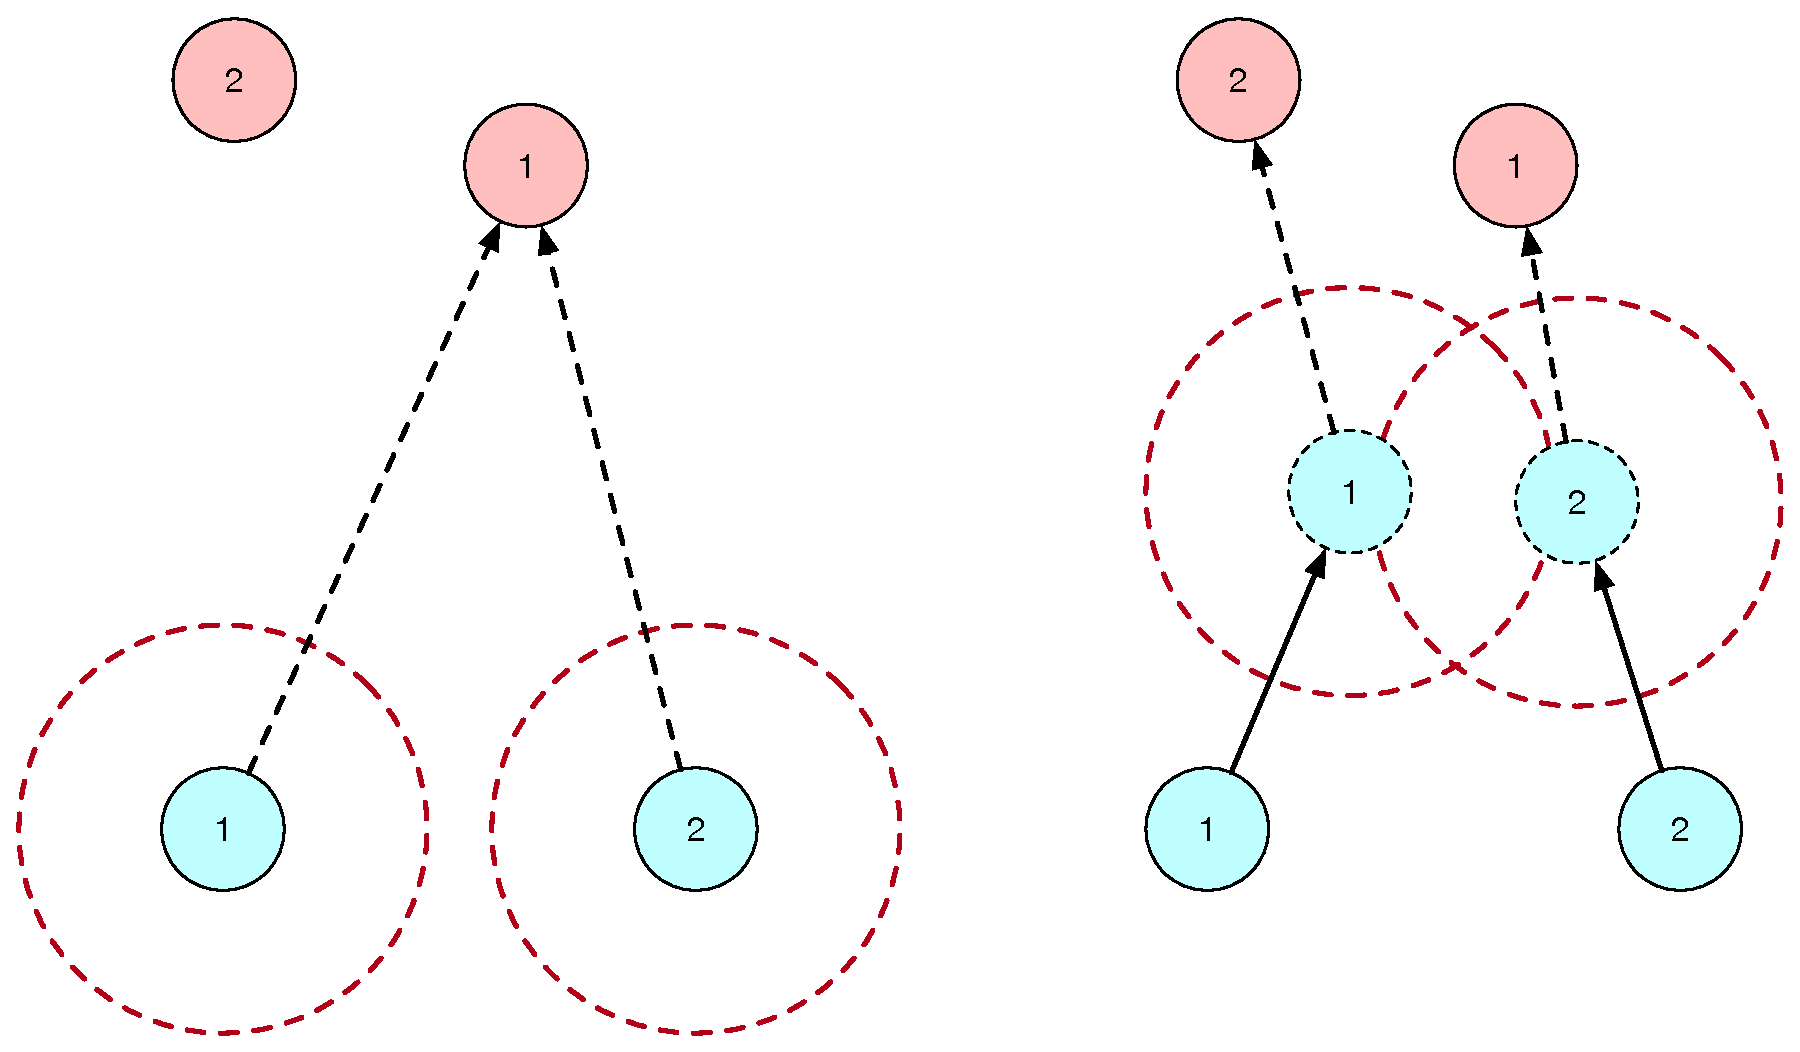
\includegraphics[height=6cm]{stochastic_game/collision_resolution}
  \bicaption[非连通场景下分配冲突消解示意图]
  {非连通场景下分配冲突消解示意图}
  {Resolution of an assignment conflict in the disconnected communication scenes}
  \label{fig:collision_resolution}
\end{figure}

\subsection{目标数量变化}
\label{special:target_num_change}

目标数量变化可分为目标数量增加和目标数量减少两种场景。目标增加的原因通常有两种:一是导弹发射前已知该目标,但导弹发射后该目标处于导弹探测区外,随着攻击过程的进行才进入导弹探测范围;二是导弹发射前该目标未出现或未被地面雷达或载机捕捉,在导弹飞行过程中被导弹自行捕获。本文不考虑原先被跟踪的目标逃出导弹探测范围的情况,因此目标减少的原因通常就是被导弹击中。

针对目标增加的第一种原因,由于导弹在发射前对于目标数量等信息已知,因此只需结束当前博弈阶段,触发重分配机制,建立新的博弈阶段并求解新的分配解即可,为了使得新探测到的目标进入分配解,在建立新博弈阶段时,首先发现该目标的导弹在确定初始解时不再使用式(\ref{sg:eq:crossfactor})所示的交叉算子,而是直接使用新目标作为初始解,由于在原分配中没有导弹选择新目标,因此在分配模型中新目标将会被保留,只能在导弹之间交换而不会被某个导弹单方面放弃。

针对目标增加的第二种原因,由于第\ref{chap:model}章模型建立中式(\ref{model:eq:bmax})的约束,因此在之前的讨论中导弹数量往往不会多于攻击所有已有目标所需的数量之和,而没有多余的导弹攻击新增的目标。假设新目标$\mathcal{T}_w$所需的导弹数量为$b_{\text{max}}^{(w)}$,在不考虑发射新的导弹的情况下,解决这一问题的方案是是改变现有模型,从原分配解中满足$b_{\text{max}}^{(j)}>1$的目标的攻击导弹中抽出$b_{\text{max}}^{(w)}$个导弹,用于攻击新目标\footnote{显然这种方案成立的条件是$n_m-n_t \geq b_{\text{max}}^{(w)}$,本文的讨论是基于满足该条件的场景下,对于不满足该条件的场景,本文不再讨论。}。

针对目标减少的场景,往往是由于导弹击中目标,因此也包含着导弹数量减少的场景。本章建立的模型中,导弹击中目标的判定条件是弹目距离小于指定阈值$R_{\text{min}}$代表目标进入导弹杀伤范围,或弹目相对接近速度$V_R>0$,代表弹目距离不再减小。此时击中目标数量若达到$b_{\text{max}}^{(j)}$,则目标被击落,攻击该目标的导弹也退出通信网络与分配模型。当一些导弹攻击完成后,其邻居节点可能失去连接通道,从而不再连通,此时将回到\ref{special:disconnected_network}小节中所论述的场景。

\section{动态任务分配系统流程}

结合\ref{sg:framework}节和\ref{sg:special_incidence}节的内容,图给出了动态环境下基于随机博弈模型的任务分配系统框图。

\begin{figure}[!htp]
  \centering
  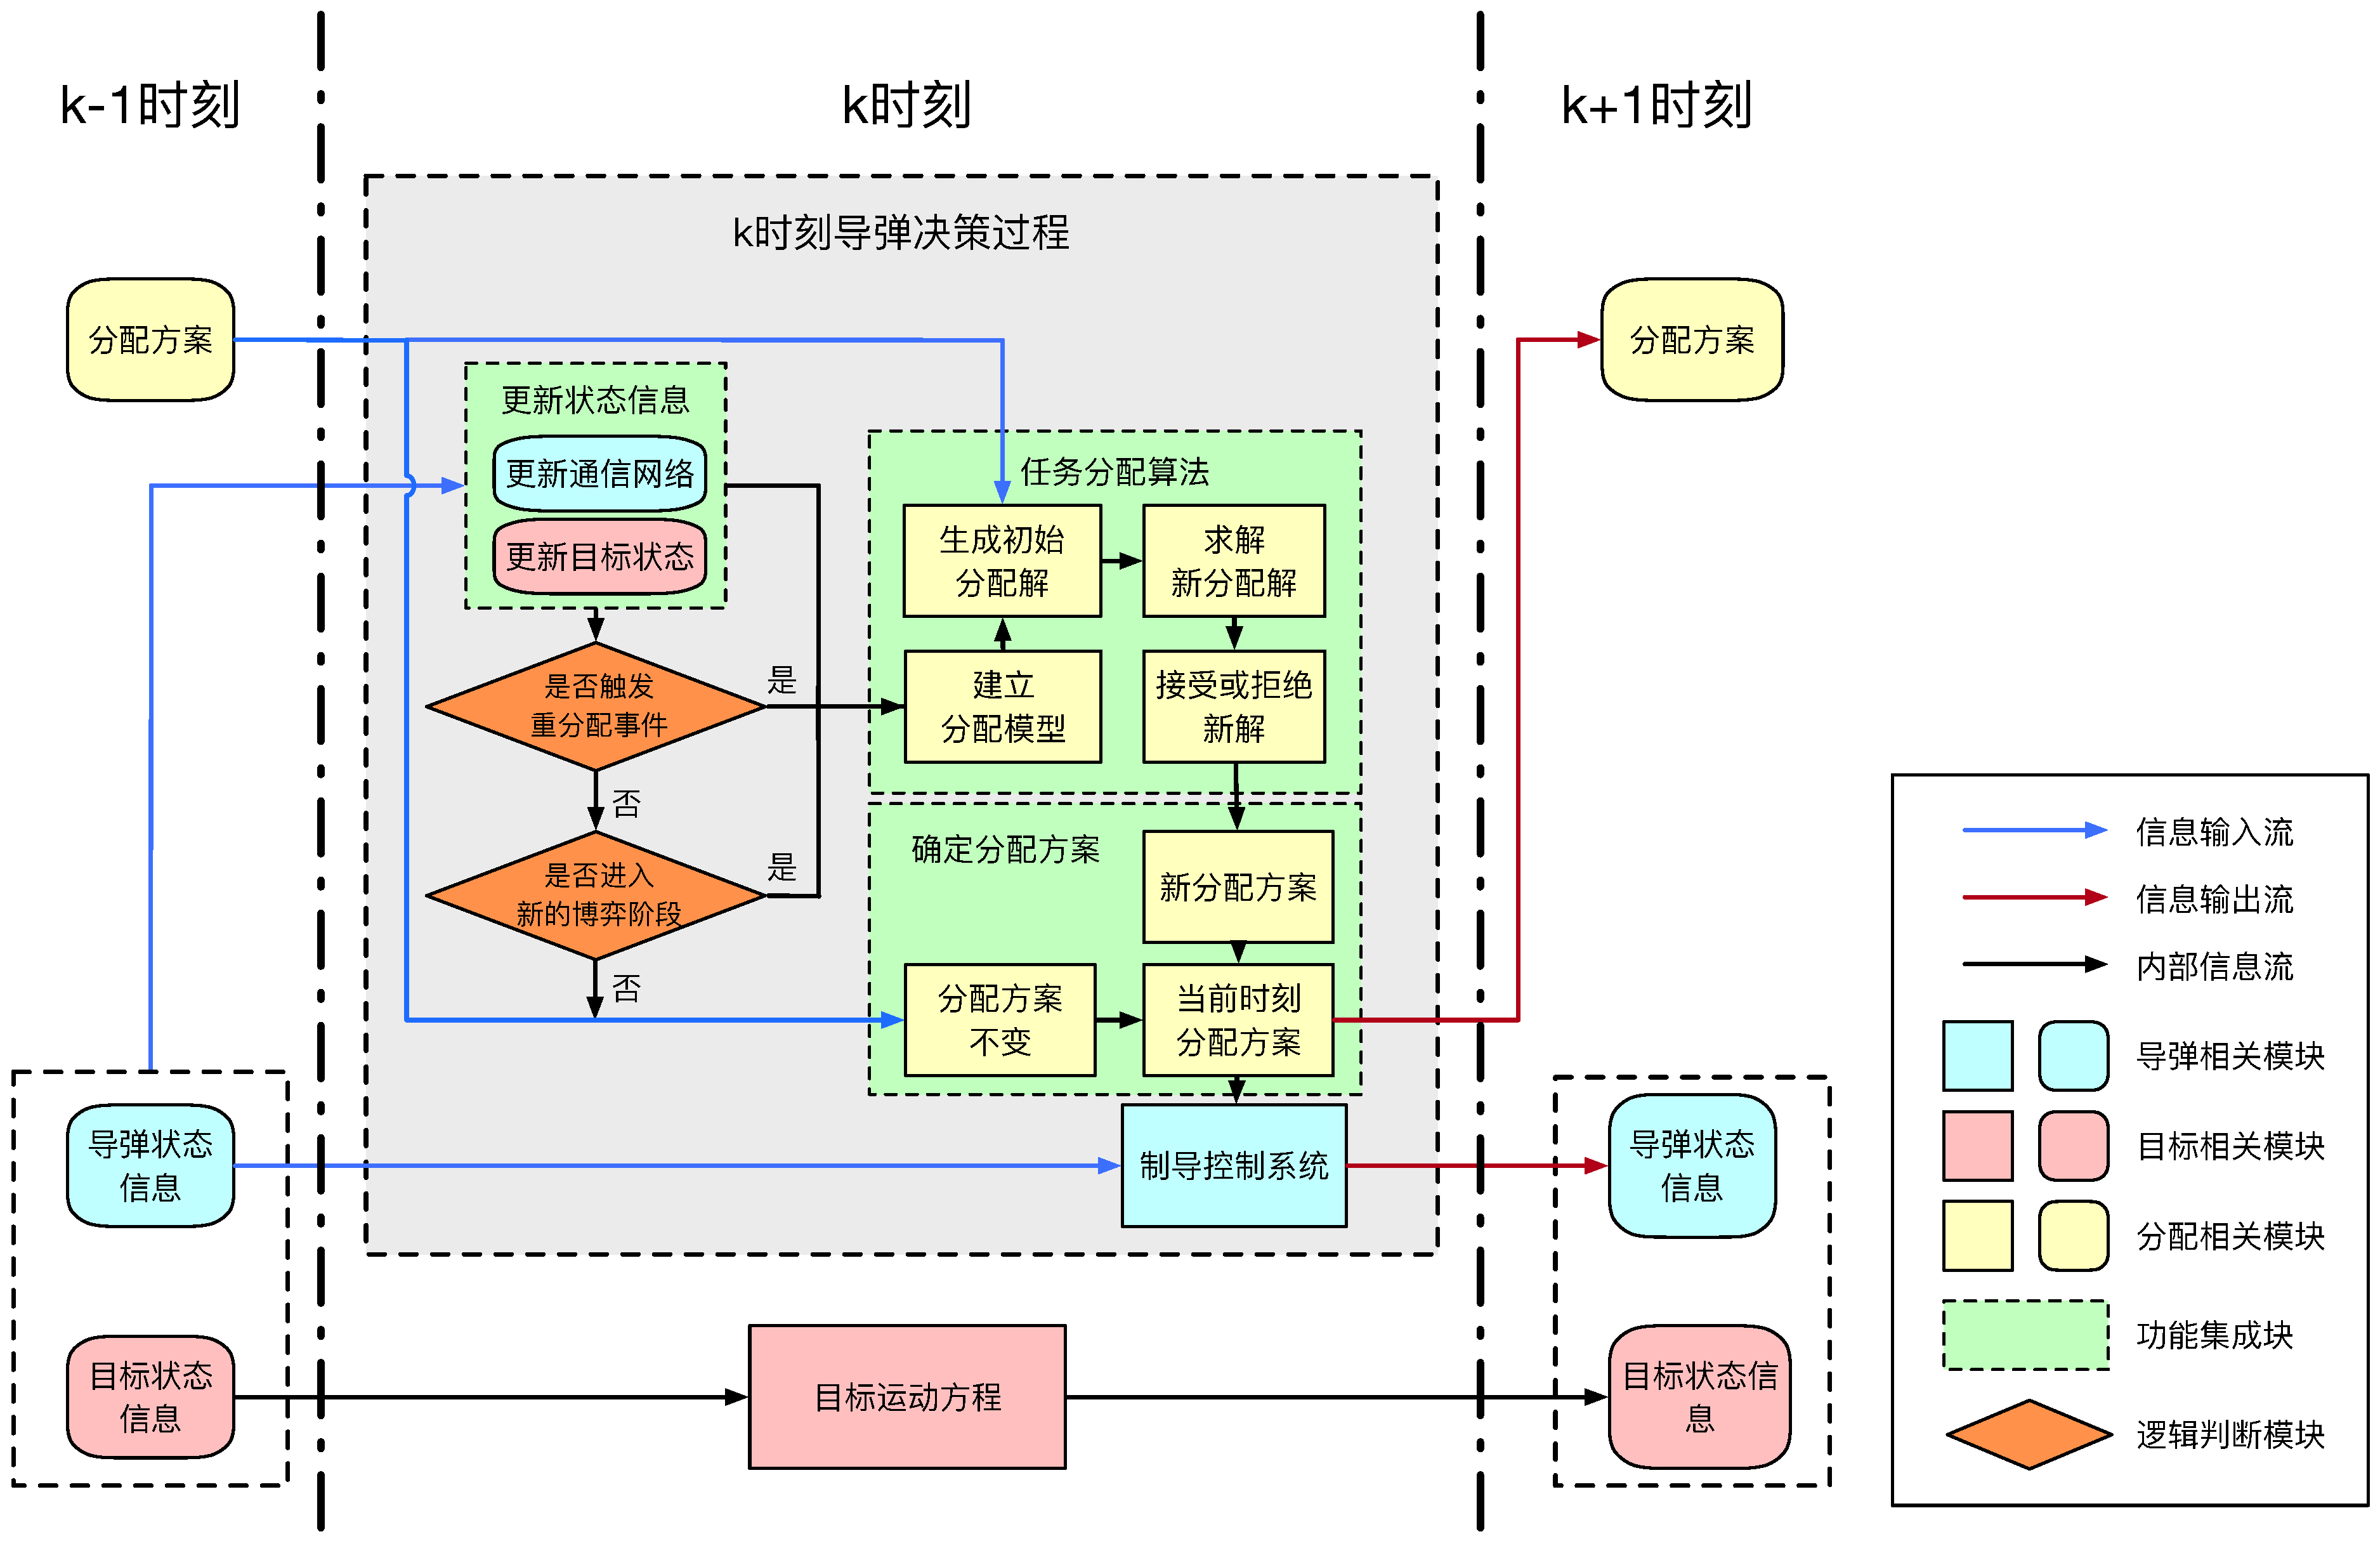
\includegraphics[height=10cm]{stochastic_game/framework}
  \bicaption[导弹任务分配系统框架示意图]
  {导弹任务分配系统框架示意图}
  {Illustration of framework of missiles task assignment system}
  \label{fig:framework}
\end{figure}

其中目标运动部分独立在外,不在控制范围内。导弹模块主要分为态势信息收集与更新、事件触发判断、任务分配和制导控制四个模块,各部分的主要功能为:

(1)态势信息收集与更新。在每个时刻导弹需要获知自身状态信息与可选目标信息,并寻找可建立通信关系的同伴,建立通信网络,共享目标信息。

(2)事件触发判断部分实现的功能是根据当前时刻收集到的导弹与目标状态信息,判断是否发生了需要立即重新分配的事件。根据上文的讨论,这些事件主要包括导弹通信网络的改变、新目标的出现和目标被导弹击中等场景。发现事件发生的导弹立即进入重分配过程,并将事件情况向可通信导弹发出,促使其他导弹也进入重分配过程。

(3)任务分配部分在两种场景下会被调用。一种是正常的博弈阶段结束,进入下一阶段时会获取新态势进行新的任务分配过程;另一种则是根据事件触发判断部分的结果,在正常阶段结束前提前进入重分配过程。该部分的主要流程是根据获取的态势建立分配模型,同时利用\ref{game_stage:stage_transform}小节中提出的初始解生成方法,生成代入求解模型的初始分配,在得到当前态势下收敛的分配解后,再以一定概率接受或拒绝该分配。

(4)制导控制部分负责根据导弹计算出的分配结果,计算制导制令,并控制导弹向指定的目标飞去。

在每个时间点,导弹不断重复以上四个步骤,直到该导弹击中目标即停止。当所有导弹均击中目标时,整个导弹集群任务分配系统停止运行。

\section{仿真对比与分析}

\section{本章小结}
\label{reassign:sec:conclusion}

